\documentclass{ctexart}
    \usepackage{mathrsfs}
    \usepackage{multirow}
    \usepackage{graphicx}
    \usepackage{array}
    \usepackage{makecell}
    \usepackage{amsmath}
    \usepackage{booktabs}
    \usepackage{float}
    \usepackage{diagbox}
    \newcommand\mgape[1]{\gape{$\vcenter{\hbox{#1}}$}}
    \newcommand\Ronum[1]{\uppercase\expandafter{\romannumeral #1\relax}}
    \newcommand\ronum[1]{\romannumeral #1\relax}
    \author{钱思天\ 1600011388 No.8}
    \title{实验九\ 刚体转动实验 \ 实验报告}
    \begin{document}
      \maketitle
      \section{实验数据与处理}
      \subsection{测量数据列表}
      \subsubsection{实验内容(2)}
      测量数据列表如下:
      % Table generated by Excel2LaTeX from sheet 'Sheet1'
\begin{table}[H]
  \centering
  \caption{$h=86.00cm,r=2.505cm$}
  \resizebox{\textwidth}{!}
  {
    \begin{tabular}{|c|c|c|c|c|c|c|}\hline
    {添加砝码质量$\Delta m_i/g$} & {总砝码质量$m_i/g$} & {$t_1/s$} & {$t_2/s$} & {$t_3/s$} & {$\bar{t}/s$} & {$t^{-2}/s^{-2}$} \\\hline
    4.99  & 4.99  & 17.63 & 17.65 & 17.63 & 17.64 & 0.003215 \\\hline
    5.00  & 9.99  & 11.13 & 11.16 & 11.12 & 11.14 & 0.008063 \\\hline
    4.98  & 14.97  & 8.85  & 8.98  & 8.95  & 8.93  & 0.012549 \\\hline
    5.01  & 19.98  & 7.50  & 7.50  & 7.50  & 7.50  & 0.017778 \\\hline
    5.02  & 25.00  & 6.65  & 6.72  & 6.62  & 6.66  & 0.022523 \\\hline
    5.01  & 30.01  & 6.00  & 6.00  & 6.00  & 6.00  & 0.027778 \\\hline
    4.98  & 34.99  & 5.62  & 5.60  & 5.62  & 5.61  & 0.031736 \\\hline
    \end{tabular}%
  }
  \label{tab:addlabel}%
\end{table}%

      \subsubsection{实验内容(3)}
      测量数据表格如下:
      % Table generated by Excel2LaTeX from sheet 'Sheet1'
\begin{table}[H]
  \centering
  \caption{$m=19.98g,h=86.00cm$}
    \begin{tabular}{|c|c|c|c|c|c|c|}\hline
    {半径$r/cm$} & {$t_1/s$} & {$t_2/s$} & {$t_3/s$} & {$\bar{t}/s$} & {$t^{-2}/s^{-2}$} & {$r^{-1}t^{-2}/s^{-2}cm^{-1}$} \\\hline
    1.001  & 18.82 & 18.81 & 18.85 & 18.83 & 0.002821 & 0.002819 \\\hline
    1.495  & 12.71 & 12.73 & 12.79 & 12.74 & 0.006158 & 0.004119 \\\hline
    2.000  & 9.55  & 9.53  & 9.49  & 9.52  & 0.011026 & 0.005513 \\\hline
    2.505  & 7.51  & 7.56  & 7.53  & 7.53  & 0.017621 & 0.007034 \\\hline
    3.002  & 6.31  & 6.29  & 6.27  & 6.29  & 0.025275 & 0.00842 \\\hline
    \end{tabular}%
  \label{tab:addlabel}%
\end{table}%

      \subsubsection{实验内容(4)}
      测量数据表格如下:
      % Table generated by Excel2LaTeX from sheet 'Sheet1'
\begin{table}[H]
  \centering
  \caption{$h=86.00cm,r=2.505cm,m=10.01g$}
    \begin{tabular}{|c|c|c|c|c|c|c|}\hline
    {$x_i/cm$} & {$t_1/s$} & {$t_2/s$} & {$t_3/s$} & {$\bar{t}/s$} & {$t^2/s^2$} & {$x_i^2/cm^2$} \\\hline
    3.354 & 6.56  & 6.41  & 6.47  & 6.48  & 41.9904 & 11.24932 \\\hline
    5.777 & 7.44  & 7.44  & 7.53  & 7.47  & 55.8009 & 33.37373 \\\hline
    8.163 & 8.62  & 8.59  & 8.53  & 8.58  & 73.6164 & 66.63457 \\\hline
    10.792 & 10.04 & 9.99  & 9.91  & 9.98  & 99.6004 & 116.4673 \\\hline
    13.041 & 11.16 & 11.2  & 11.12 & 11.16 & 124.5456 & 170.0677 \\\hline
    \end{tabular}%
  \label{tab:addlabel}%
\end{table}%

      \subsection{实验数据处理}
      \subsubsection{验证线性关系}
      根据实测数据,可分别作图如下:
      \begin{figure}[H]
        \centering
        \caption{$t^{-2}-m$散点及趋势线图}
        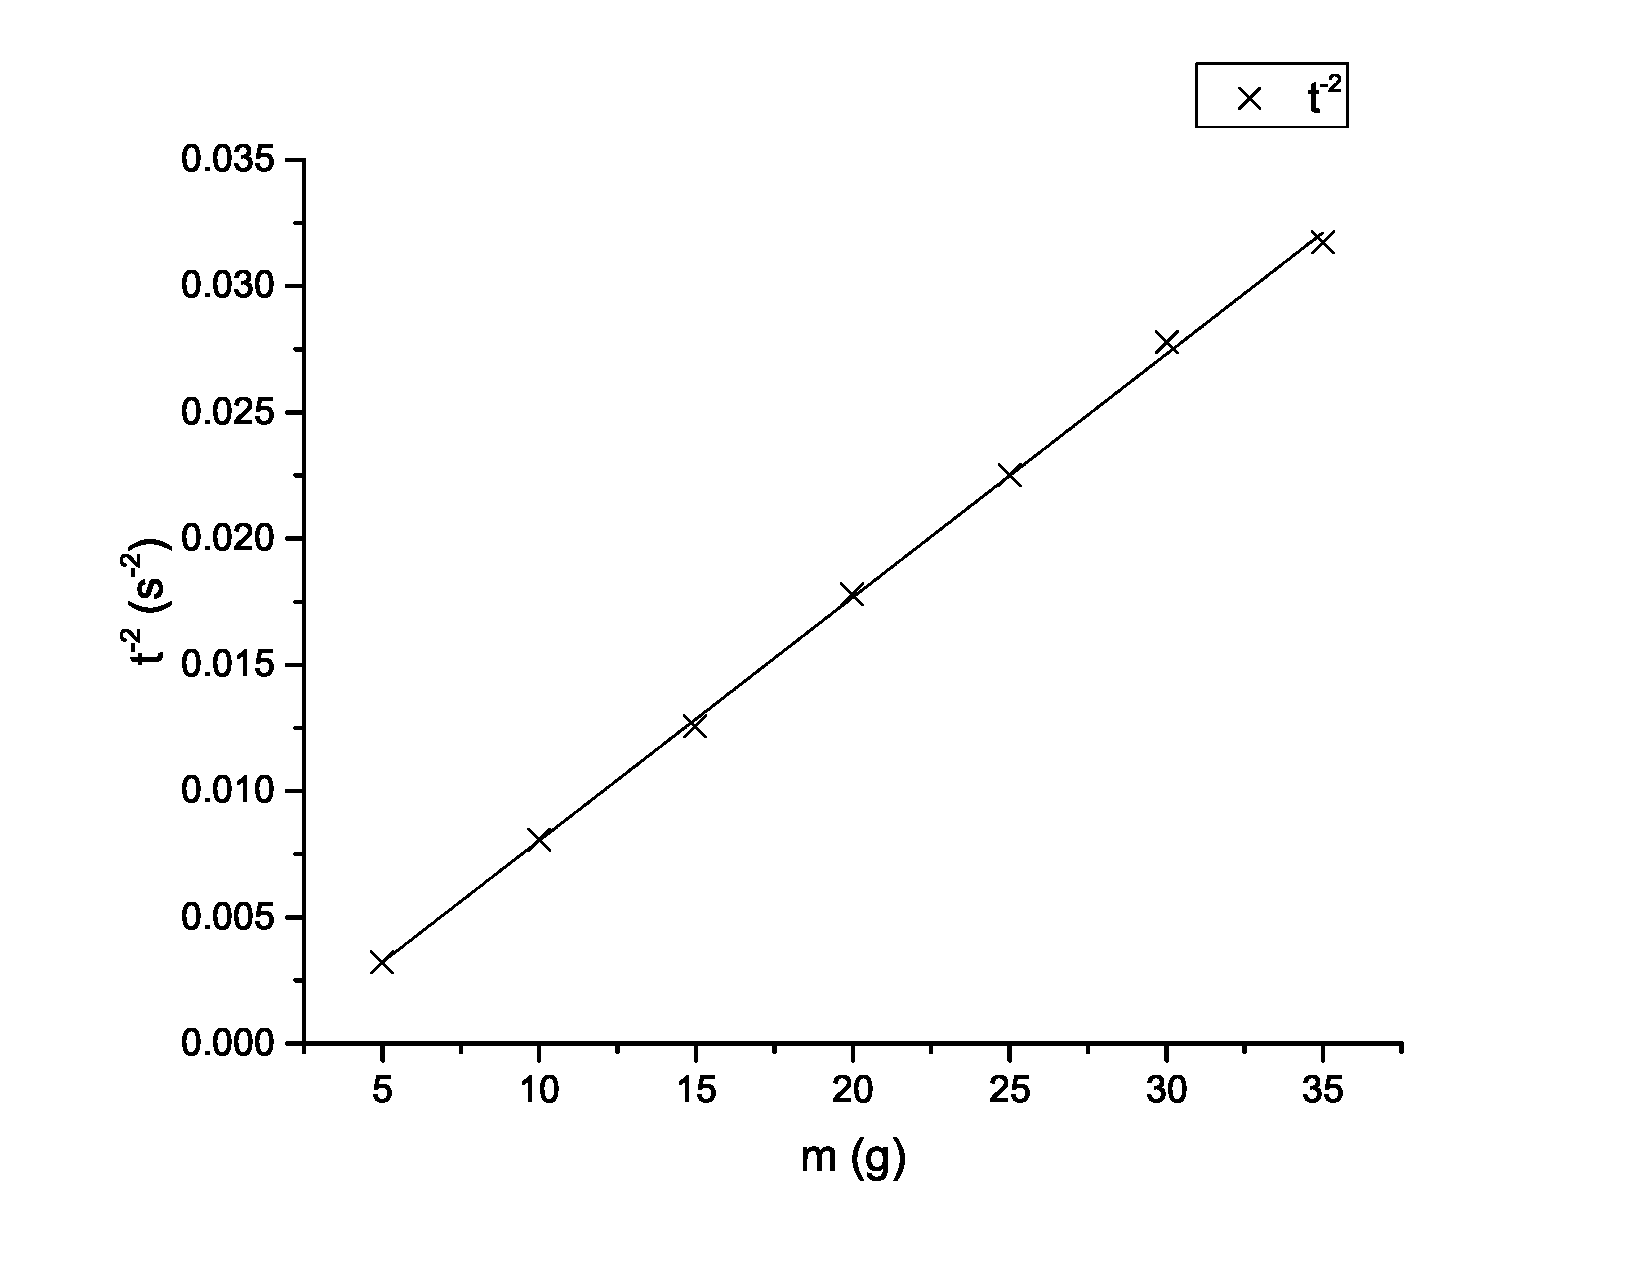
\includegraphics[width=1.0\textwidth]{1}
        \label{fig:digit}
      \end{figure}
      计算得相关系数为:$R\approx0.9997$;可以看出(1)在$r$一定的情况下,$t^{-2}$与$r$成线性关系.
      \begin{figure}[H]
        \centering
        \caption{$r^{-1}t^{-2}-r$散点及趋势线图}
        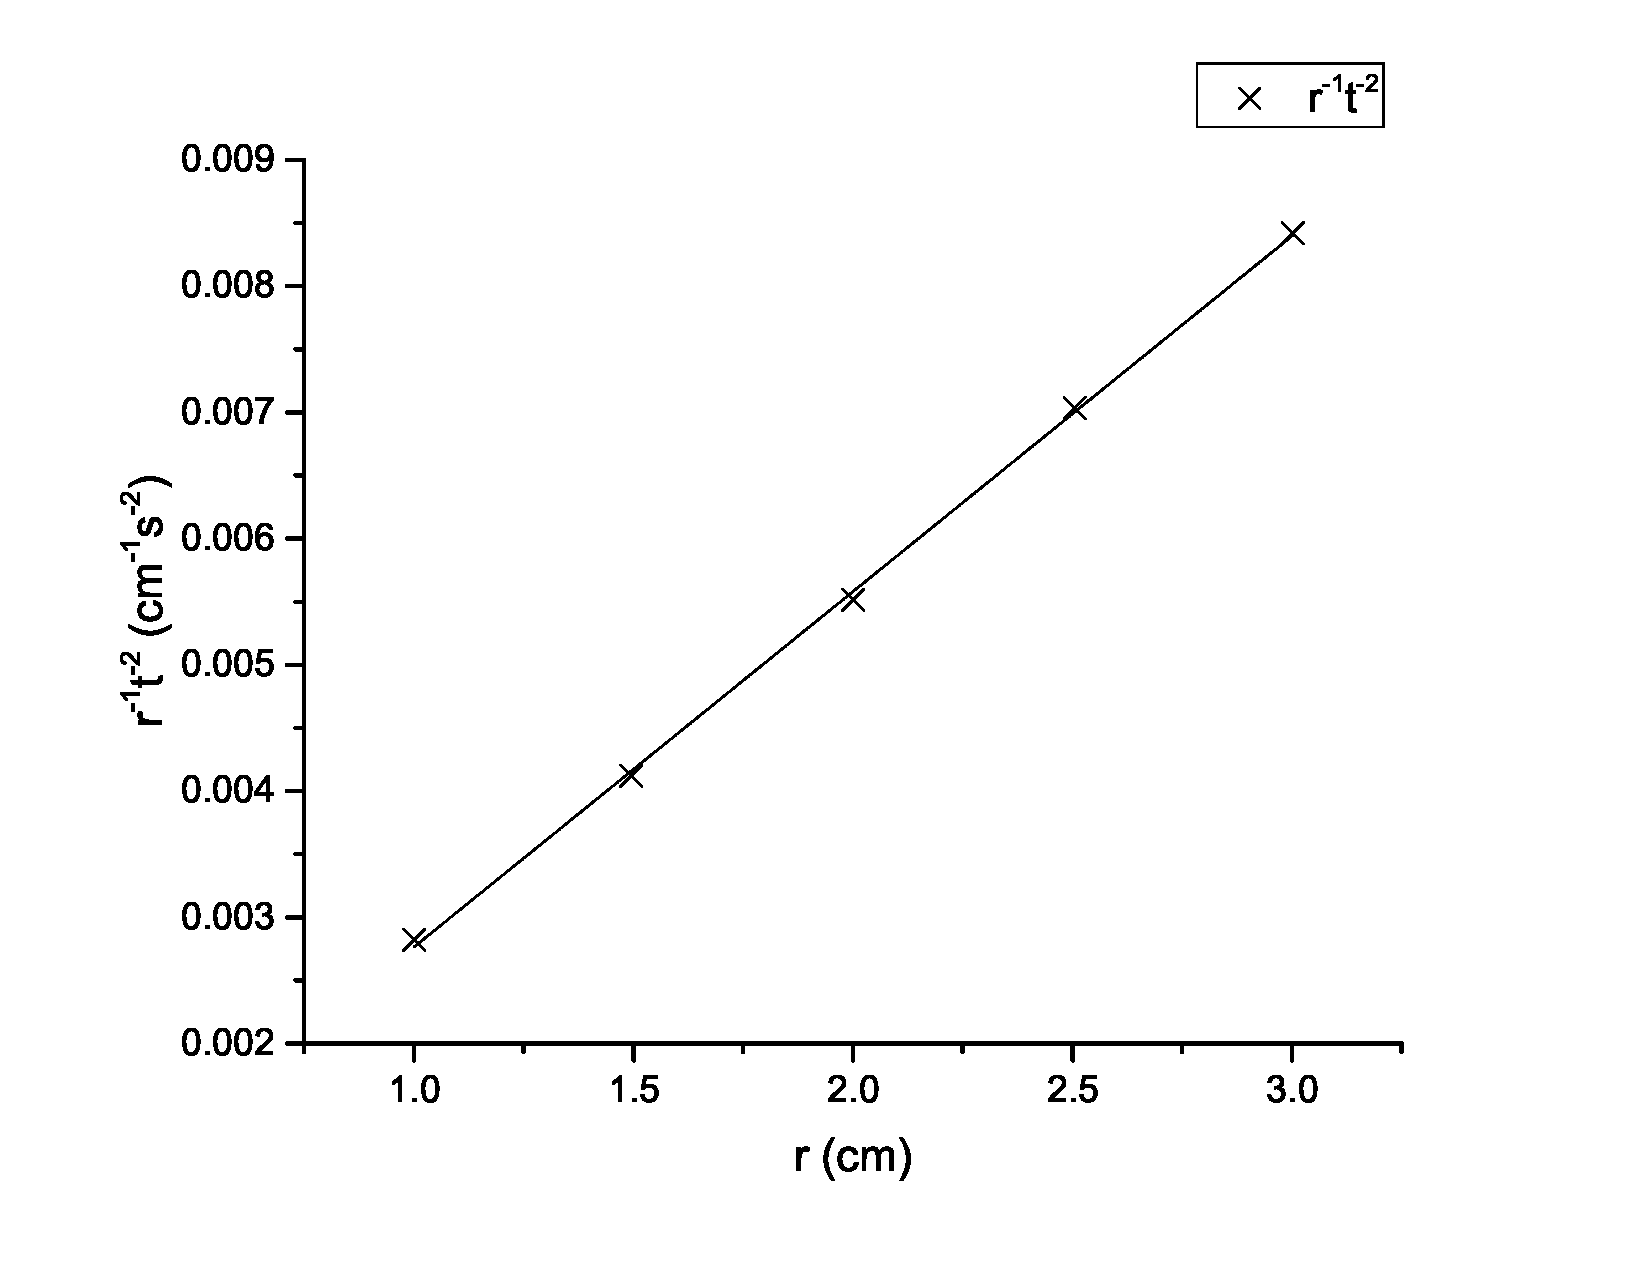
\includegraphics[width=1.0\textwidth]{2}
        \label{fig:digit}
      \end{figure}
      计算得相关系数为:$R\approx0.9998$;     
      可以看出(2)在$m$一定的情况下,$t^{-2}r^{-1}$与$r$成线性关系。
      \begin{figure}[H]
        \centering
        \caption{$t^2-x_i^2$散点及趋势线图}
        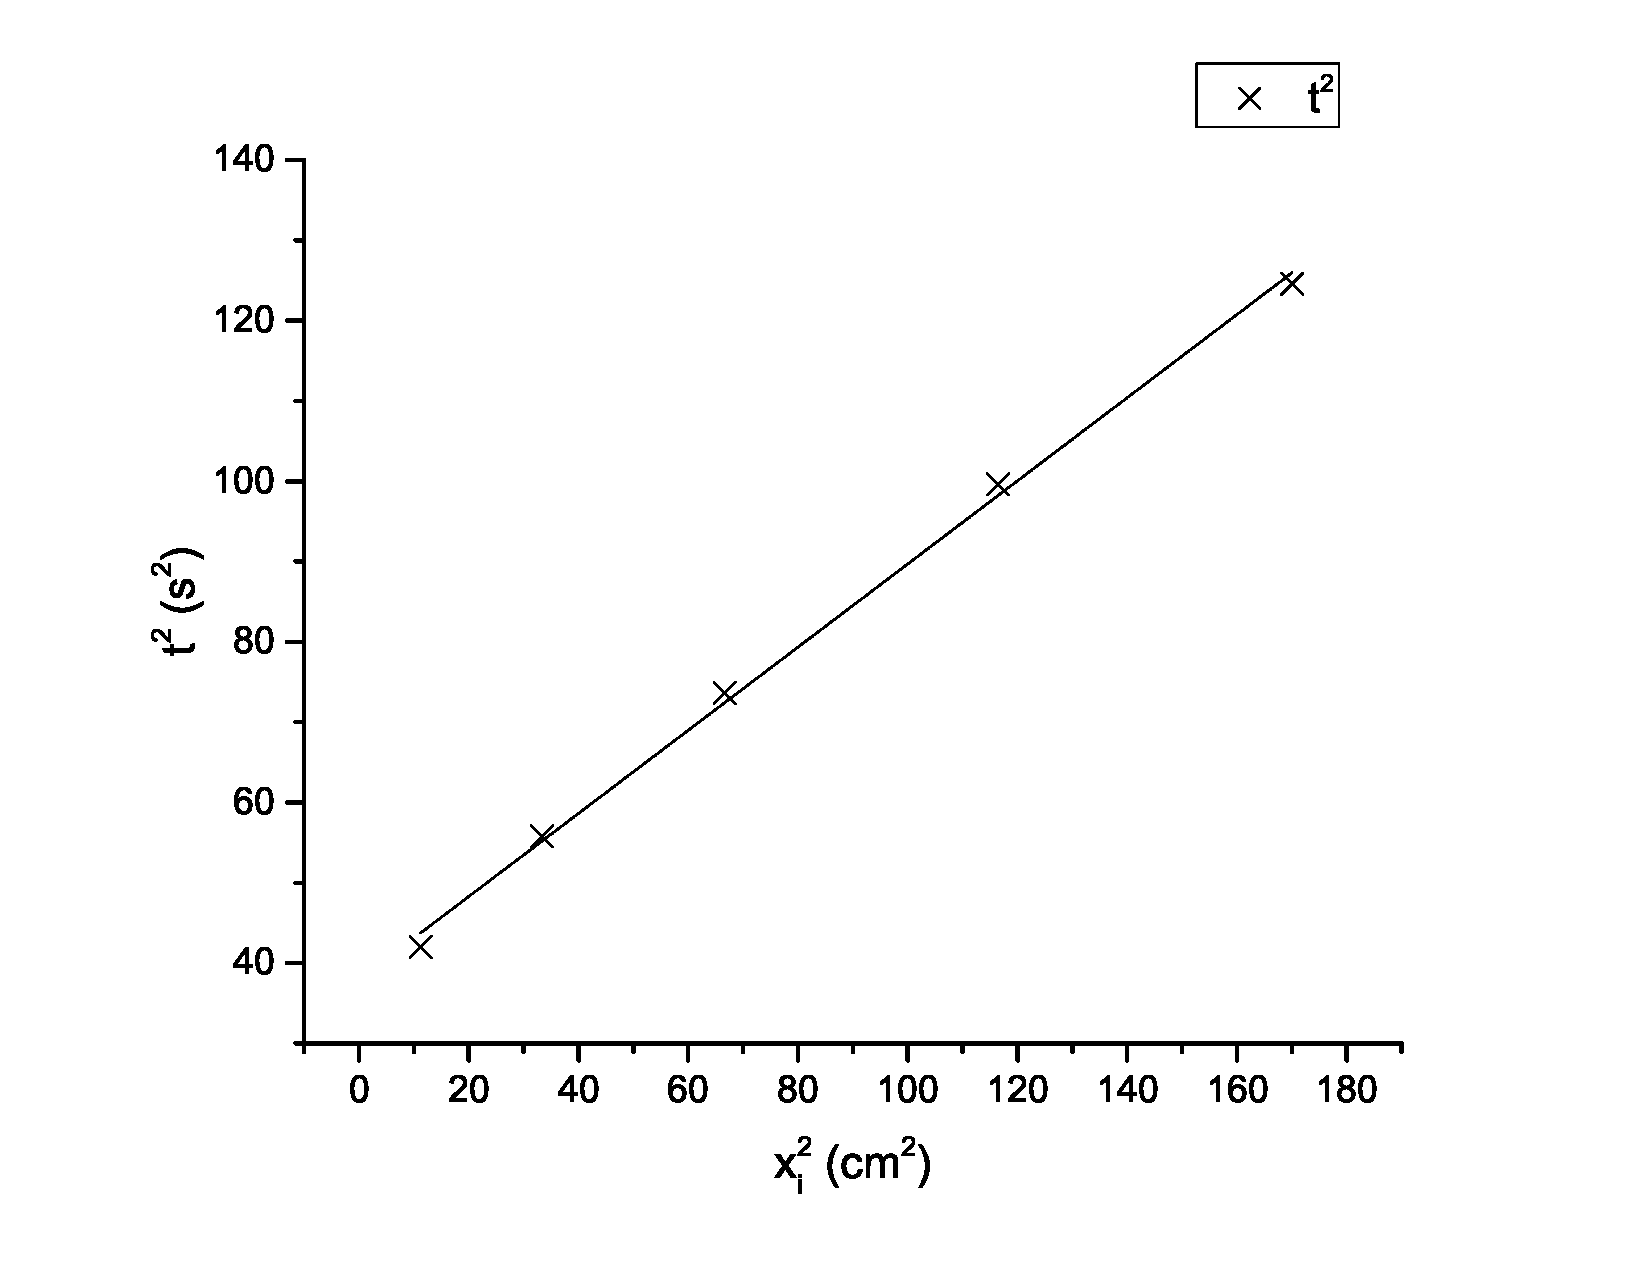
\includegraphics[width=1.0\textwidth]{3}
        \label{fig:digit}
      \end{figure}
      计算得相关系数为:$R\approx0.9990$
      
      从图中,可得$t^2$与$x^2$确实存在线性关系,这也验证了平行轴定理。
      \subsubsection{线性拟合求转动惯量}
      对于实验(2):

      采用最小二乘法,设:$$t^{-2}=k_1m+b_1$$
      
      则有公式:$$k_1=\frac{\sum\limits_{i=1}^7{(t_i^{-2}-\bar{t}^{-2})}(m_i-\bar{m})}{\sum\limits_{i=1}^7{(m_i-\bar{m})^2}}=9.636\times10^{-4}(g^{-1}s^{-2})$$

      下计算$k_1$的不确定度,分为两项:
      
      A类不确定度:其计算可利用:$$\frac{\sigma_{k_1A}}{k_1}=\sqrt{\frac{R^{-2}-1}{7-2}}\Rightarrow\sigma_{k_1A}=1.1\times10^{-5}(g^{-1}s^{-2})$$

      B类不确定度:根据$k_1$的计算公式,可得$$\sigma_{k_2B}=\sqrt{\sum\limits_{i=1}^7({\frac{(m_i-\bar{m})\sigma_{t^{-2}_i}}{\sum\limits_{i=1}^7{(m_i-\bar{m})^2}}})^2}$$,理论上,应代入不同的$\sigma_{t^{-2}_i}$值,但为了计算方便,我取$\sigma_{t_i^{-2}}$的最大值代入计算,事实上这一数值也能反应实验偏差的最大限度。
      而对于$\sigma_{t_i^{-2}}$的计算,首先应计算$t_i$的不确定度再进行传递,$t_i$的不确定度为两项的叠合,一项是秒表的允差$\sigma_B=\frac{e_t}{\sqrt{3}}$,另一项是平均值的标准偏差$\sigma_A=\sqrt{{\frac{\sum\limits_{i=1}^3(t_i-\bar{t})^2}{2\times3}}}$。经计算$\sigma_{t^{-2}}^{MAX}=9.9723\times10^{-5}(s^{-2})$。故$\sigma_{k_1B}=3.7672\times10^{-6}{g^{-1}s^{-2}}$。

      综上,得$$\sigma_{k_1}=1\times10^{-5}(g^{-1}s^{-2})$$

      故$$k_1\pm\sigma_{k_1}=(9.6\pm0.1)\times10^{-4}(g^{-1}s^{-2})$$

      $$h\pm\sigma_h=86.0\pm0.6(cm)$$

      $$r\pm\sigma_r=2.505\pm0.001(cm)$$

      根据公式$$I_1=\frac{gr^2}{2hk_1}=3.710\times10^{-3}(kg\cdot m^3)$$

      $$\frac{\sigma_{I_1}}{I_1}=\sqrt{(\frac{2\sigma_r}{r})^2+(\frac{\sigma_h}{h})^2+(\frac{\sigma_{k_1}}{k_1})^2}$$

      得:$$\sigma_{I_1}=2\times10^{-4}(kg\cdot m^3)$$

      $$I_1\pm\sigma_{I_1}=(3.7\pm0.2)\times10^{-3}(kg\cdot m^3)$$
      
      对于实验(3):

      采用最小二乘法,设:$$r^{-1}t^{-2}=k_2r+b_2$$
      
      则有公式:$$k_2=\frac{\sum\limits_{i=1}^7{((r^{-1}t^{-2})_i-\bar{t}^{-2})}(m_i-\bar{m})}{\sum\limits_{i=1}^7{(m_i-\bar{m})^2}}=2.82\times10^{-3}(cm^{-2}s^{-2})$$

      下计算$k_2$的不确定度,分为两项:
      
      A类不确定度:其计算可利用:$$\frac{\sigma_{k_2A}}{k_2}=\sqrt{\frac{R^{-2}-1}{5-2}}\Rightarrow\sigma_{k_2A}=3.646\times10^{-5}(cm^{-2}s^{-2})$$

      B类不确定度:根据$k_1$的计算公式,可得$$\sigma_{k_2B}=\sqrt{\sum\limits_{i=1}^7({\frac{(m_i-\bar{m})\sigma_{t^{-2}_i}}{\sum\limits_{i=1}^7{(m_i-\bar{m})^2}}})^2}$$,理论上,应代入不同的$\sigma_{t^{-2}_i}$值,但为了计算方便,我取$\sigma_{t_i^{-2}}$的最大值代入计算,事实上这一数值也能反应实验偏差的最大限度。
      而对于$\sigma_{t_i^{-2}}$的计算,首先应计算$t_i$的不确定度再进行传递,$t_i$的不确定度为两项的叠合,一项是秒表的允差$\sigma_B=\frac{e_t}{\sqrt{3}}$,另一项是平均值的标准偏差$\sigma_A=\sqrt{{\frac{\sum\limits_{i=1}^3(t_i-\bar{t})^2}{2\times3}}}$。经计算$\sigma_{t^{-2}}^{MAX}=9.9723\times10^{-5}(s^{-2})$。故$\sigma_{k_1B}=3.7672\times10^{-6}{g^{-1}s^{-2}}$。

      综上,得$$\sigma_{k_1}=1\times10^{-5}(g^{-1}s^{-2})$$

      故$$k_1\pm\sigma_{k_1}=(9.6\pm0.1)\times10^{-4}(g^{-1}s^{-2})$$

      $$h\pm\sigma_h=86.0\pm0.6(cm)$$

      $$r\pm\sigma_r=2.505\pm0.001(cm)$$

      根据公式$$I_1=\frac{gr^2}{2hk_1}=3.710\times10^{-3}(kg\cdot m^3)$$

      $$\frac{\sigma_{I_1}}{I_1}=\sqrt{(\frac{2\sigma_r}{r})^2+(\frac{\sigma_h}{h})^2+(\frac{\sigma_{k_1}}{k_1})^2}$$

      得:$$\sigma_{I_1}=2\times10^{-4}(kg\cdot m^3)$$

      $$I_1\pm\sigma_{I_1}=(3.7\pm0.2)\times10^{-3}(kg\cdot m^3)$$
      \section{分析与讨论}
      \subsection{减少误差}
      \paragraph{系统误差}为减少系统误差,应尽量满足得出实验结论所需的一系列近似条件;同时,应使$OO_1$轴尽量竖直,绳子尽量水平以及让绳子密绕
      在塔轮上等。
      \paragraph{随机误差}掐秒表时应集中注意力,找准落地点等。
      \subsection{思考题(5)}
      实验(3)中,考虑塔轮半径的改变,其摩擦力矩$M_{\mu}$改变且越来越大,因此有:
      $$(mg-f)r-M_{others}=I\dot\omega=\frac{2hI}{rt^2}$$
      $$\Rightarrow I_2=\frac{mgk}{2h}=\frac{mg}{mg-f}I>I$$
      同时,实验(2)中,塔轮半径不变,因此摩擦力矩$M_{\mu}$可认为不变,故可认为$I_1=I$,
      则有$I_2>I_1$。
      \section{收获与感想}
      在预习这个实验的时候,我情不自禁地想起来高一时所做的,验证牛顿第二定律的实验,也是用重物的重力做外力并计算加速度。

      在我看来,这两个实验有很多相似的地方,譬如都要使加速度远小于重力加速度等。

      其实从实验研究的对象,也能感受到高中与大学所学习内容的区别,从可当作质点运动的整体平动,到刚体的转动,我们所学习的物理也更加高深了。

      此外,在本次实验中,我也感受到了自己某些实验能力还有不足,例如对秒表的掌控等,希望在以后的实验课程中,能够提高自己的实验能力。

\end{document} 